\section{实验}

\subsection{实验设置}

\begin{table*}[!t]
\centering
\small
\setlength{\tabcolsep}{5pt}
\renewcommand{\arraystretch}{1.1}
\begin{threeparttable}
\caption{在不同模型下，\our 与基线智能体系统在 GAIA、Terminal-Bench 2.0 和 SWE-Bench-Verified 上的对比。最佳结果以\textbf{粗体}标出。}
\label{tab:main_results}
\begin{tabular}{l l cc cc cc c}
\toprule
\textbf{方法} & \textbf{模型配置}
& \multicolumn{2}{c}{\textbf{GAIA}}
& \multicolumn{2}{c}{\textbf{Terminal-Bench 2.0}}
& \multicolumn{2}{c}{\textbf{SWE-Bench-Verified}}
\\
\cmidrule(lr){3-4}\cmidrule(lr){5-6}\cmidrule(lr){7-8}
&
& \textbf{Pass@1} & \textbf{Pass@3}
& \textbf{Pass@1} & \textbf{Pass@3}
& \textbf{Pass@1} & \textbf{Pass@3}
& \textbf{平均 Pass@1}\\
\midrule

\multirow[c]{3}{*}{ReAct}
& Gemini-3-Flash     & 49.09 & 66.06 & 28.57 & 47.14 & 64.00 & 82.00 & 47.22 \\
& DeepSeek-V3.2      & 46.70 & 71.51 & 20.00 & 32.86 & 48.00 & 87.00 & 38.23 \\
& Claude-4.5-haiku   & 47.88 & 62.42 & 20.00 & 37.14 & 63.00 & 87.00 & 43.62 \\
\cmidrule(lr){1-9}

\multirow[c]{3}{*}{OpenHands}
& Gemini-3-Flash     & 66.06 & 72.73 & 31.43 & 51.43 & 48.00 & 66.00 & 48.49 \\
& DeepSeek-V3.2      & 63.64 & 72.12 & 21.43 & 35.71 & 60.00 & 75.00 & 48.35 \\
& Claude-4.5-haiku   & 54.55 & 61.21 & 12.85 & 25.71 & 68.00 & 83.00 & 45.13 \\
\cmidrule(lr){1-9}

\multirow[c]{3}{*}{Mini-SWE}
& Gemini-3-Flash     & 58.18 & 68.48 & 34.29 & 50.00 & 56.00 & 85.00 & 49.49 \\
& DeepSeek-V3.2      & 50.30 & 63.63 & 30.00 & 48.57 & \textbf{84.00} & \textbf{89.00} & 54.76 \\
& Claude-4.5-haiku   & 40.61 & 60.00 & 24.29 & 28.57 & 44.00 & 83.00 & 36.30 \\
\cmidrule(lr){1-9}

\multirow[c]{2}{*}{Claude Code}
& Gemini-3-Flash     & -- & -- & 32.86 & 48.57 & 22.00 & 42.00 & 27.43 \\
& Claude-4.5-haiku   & -- & -- & 34.29  & 45.71 & 25.00 & 41.00 & 29.65 \\
\midrule

\multirow[c]{3}{*}{\our}
& Gemini-3-Flash     & \textbf{80.00} & \textbf{86.06} & \textbf{52.86} & \textbf{57.14} & 82.00 & 86.00 & \textbf{71.62} \\
& DeepSeek-V3.2      & 67.87 & 80.00 & 31.43 & 42.86 & 76.00 & 82.00 & 58.43 \\
& Claude-4.5-haiku   & 60.61 & 73.90 & 35.71 & 45.71 & 70.00 & 84.00 & 55.44 \\
\bottomrule
\end{tabular}
\end{threeparttable}
\end{table*}

\textbf{基准。}我们在三个具有挑战性的智能体基准上评测所提出的方法，它们覆盖不同的交互环境：(1) \textbf{Terminal-Bench 2.0}~\cite{tbench_2025}，它将智能体置于带有交互式 Bash shell 的 Linux 终端中，要求执行命令行操作来完成多步现实任务；(2) \textbf{SWE-Bench-Verified}~\cite{jimenez2023swe}，它在真实 GitHub 项目上评估软件工程能力，要求智能体在真实编程环境中定位缺陷、实现补丁并通过给定测试套件；(3) \textbf{GAIA}~\cite{mialon2023gaia} 验证集，这是一个通用基准，用于测试智能体解决需要多步推理和工具使用的现实任务的能力。我们分别报告所有基准上的 pass@1 和 pass@3。附录~\ref{app:dataset} 进一步说明这些数据集的评测用法，附录~\ref{app:action_space} 则介绍每个基准所使用的工具。

\textbf{模型与基线。}
我们将所提出的方法与以下代表性框架比较：(1) \textbf{ReAct}~\cite{yao2022react}，一个直接基于 ReAct 构建、交替执行推理与动作的简单单智能体系统；(2) \textbf{OpenHands}~\cite{wang2024openhands}，一个常用于解决多类现实任务的开放智能体平台；(3) \textbf{mini-SWE-agent}~\cite{yang2024sweagent}，一个面向 GitHub issue 等任务的精简编程智能体；(4) \textbf{Claude Code}~\cite{anthropic_claude_code_subagents}，一个生产级智能体命令行工具，支持创建预定义子智能体以分解任务并隔离上下文。对于每个智能体系统，我们使用三个前沿语言模型，包括两个强模型 \texttt{Gemini-3-Flash} 和 \texttt{DeepSeek-V3.2}~\cite{liu2025deepseek}，以及一个较小模型 \texttt{Claude-4.5-haiku}。基线实现详见附录~\ref{app:baseline_imp}。

\textbf{实现。}
所有实验中，编排器的 $max\_attempt$ 设为 10，子智能体的 $max\_step$ 设为 50。为保证公平比较，所有基线的 $max\_step$ 均设为 500。免训练设置的设计详见附录~\ref{app:prompt_used}，其中给出了三个基准中使用的全部编排器和子智能体提示词。子智能体完成任务后，由一个评审 LLM 检查执行轨迹并总结核心信息。

对于 SFT 训练，我们在非思考模式下微调 Qwen3-8B~\cite{yang2025qwen3}，以增强其编排能力。我们使用 TaskCraft~\cite{shi2025taskcraft} 作为种子数据集，并用 Gemini-3-Flash 收集 2K 条编排轨迹进行 SFT 训练。SFT 阶段使用 LLaMAFactory 框架~\cite{zheng2024llamafactory} 进行 2 个 epoch 的全参数微调，学习率为 1e-5。更多细节见附录~\ref{app:sft_hyper}。

对于上下文内学习，我们使用 \texttt{Claude Sonnet 4.5} 作为优化模型，迭代更新编排器指令。实验执行 5 轮优化，每轮收集 6 条交互轨迹用于分析。每轮结束后，选取成本与性能权衡最优的提示词，即以更低成本获得最高性能的提示词，作为下一轮的初始化。

\subsection{主要结果}
\label{sec:main_results}
表~\ref{tab:main_results} 给出了 \our 与基线智能体系统在 GAIA、Terminal-Bench 2.0 和 SWE-Bench-Verified 三个基准上的主要结果，评测指标为 pass@1/pass@3。对于 \our，我们使用 \texttt{Gemini-3-Flash} 作为编排器；为便于比较，此处只提供一个模型作为子智能体选项。总体来看，\our 在所有环境中均持续优于基线。使用 \texttt{Gemini-3-Flash} 时，\our{} 在三个基准上的平均 pass@1 比最佳基线高 $22.13\%$。

\paragraph{GAIA 结果。}
GAIA 衡量通用智能体解决现实任务的能力，包括多跳搜索、文件处理和多模态操作。在这一环境中，\our 相比所有基线取得了最佳性能。具体而言，当编排器和子智能体均使用 \texttt{Gemini-3-Flash} 时，\our 的 pass@1 为 80.00，pass@3 为 86.06，优于所有基线。在相同的 \texttt{Gemini-3-Flash} 主干模型下，\our 将 pass@1 从最强基线框架 \texttt{OpenHands} 的 66.06 提升至 80.00，绝对提高 13.94 个百分点。即使使用能力较弱的 \texttt{Claude-4.5-haiku} 作为子智能体模型，它在 GAIA 上仍达到 60.61 pass@1，说明性能提升并不局限于能力最强的模型配置。由于 Claude Code 被设计为生产级编程智能体，我们未在 GAIA 上评测它，因此相应结果留空。GAIA 案例研究见附录~\ref{app:case_study}。

\paragraph{Terminal-Bench 2.0 结果。}
Terminal-Bench 评估智能体在受现实工作流启发的计算机终端环境中的操作能力。在该基准上，采用 \texttt{Gemini-3-Flash} 的 \our 取得 52.86 pass@1 和 57.14 pass@3。与表~\ref{tab:main_results} 中 pass@1 为 34.29 的最强基线 \texttt{Mini-SWE} 相比，pass@1 绝对提升 64.29 个百分点。除 \texttt{Gemini-3-Flash} 配置外，\our 在其他主干模型下仍具竞争力，其性能与 \texttt{Claude Code} 等专用编程智能体系统相当或更好。

\paragraph{SWE-Bench-Verified 结果。}
SWE-Bench-Verified 通过要求智能体为开源仓库中的真实问题生成能够通过给定测试的代码补丁，评估其解决实际问题的能力。在该基准上，\our 在不同主干模型下均表现强劲，并可与最优基线系统竞争。使用 \texttt{Gemini-3-Flash} 时，\our 达到 82.00 pass@1 和 86.00 pass@3，优于相同模型设置下的 \texttt{ReAct} 和 \texttt{OpenHands}。与专门面向软件任务的 \texttt{Mini-SWE} 相比，\our 仍具竞争力，并且在三个模型主干上均稳定达到超过 70.00 的 pass@1。

\subsection{\our 的优势分析}
\label{subsec:adv}
本节分析 \our 动态创建专用子智能体的优势，重点关注工作记忆与能力。总体而言，我们发现，由编排器向子智能体显式传递上下文能够提升性能（第~\ref{sec:adv1} 节）；针对不同任务选择不同模型可以获得成本与性能的帕累托权衡（第~\ref{sec:adv2} 节）；多种子智能体实现也能持续改善整体性能（第~\ref{sec:adv3} 节）。

\subsubsection{优势一：上下文共享}
\label{sec:adv1}

\begin{table}[t]
\centering
\small
\setlength{\tabcolsep}{6pt}
\renewcommand{\arraystretch}{1.15}
\caption{调用子智能体时的上下文控制消融。各设置仅改变传给子智能体的 \texttt{Context} 字段，以隔离上下文继承的影响；子智能体模型、工具和系统提示均保持一致。}
\label{tab:context_control}
\begin{tabular}{l c c c c}
\toprule
\textbf{设置} & \textbf{Level 1} & \textbf{Level 2} & \textbf{Level 3} & \textbf{平均值} \\
\midrule
无上下文    & 89.47 & 81.48 & 75.00 & 86.00 \\
完整上下文  & 94.74 & 77.78 & 75.00 & 84.00 \\
\textbf{本文方法} & \textbf{100.00} & \textbf{88.89} & \textbf{75.00} & \textbf{96.00} \\
\bottomrule
\end{tabular}
\end{table}

在 \our{} 中，编排器会向每个新创建的子智能体显式、动态地传递筛选后的上下文。为评估该设计的有效性，我们将其与两个变体比较：\textbf{无上下文}，每个子智能体只接收任务指令；\textbf{完整上下文}，每个子智能体继承主智能体的全部上下文。这两种方法也常见于以往系统~\cite{sun2025scaling, anthropic_claude_code_subagents}。我们在 GAIA 上开展分析，从验证集中抽取 50 个样本。

表~\ref{tab:context_control} 表明，有必要将上下文视为子智能体的重要组成部分，并把它抽象为四元组中的一个元素。具体而言，无上下文设置由于缺失关键执行轨迹和前序步骤中的细粒度线索而失败；完整上下文设置则经常引入无关信息，加剧上下文退化。相比之下，我们的方法允许编排器只选择和压缩与任务相关的历史，从而提供更干净的上下文并取得最高分。

\subsubsection{优势二：可学习的编排器}
\label{sec:adv2}

\begin{table}[htbp]
\centering
\small
\setlength{\tabcolsep}{8pt}
\caption{主要结果。ReAct 每次运行只使用一个指定语言模型，其他系统则可以使用单模型或混合模型池。ICL 表示上下文内学习。}
\label{tab:level_main}
\resizebox{\linewidth}{!}{%
\begin{tabular}{l l c c}
\toprule
\textbf{系统} & \textbf{语言模型} & \textbf{准确率} & \textbf{平均成本} \\
\midrule

\multirow{5}{*}{ReAct}
& Claude-4.5-sonnet  & 53.93 & 0.190 \\
& Claude-4.5-haiku   & 47.88 & 0.066 \\
& Gemini-3-Flash     & 49.09 & 0.070 \\
& GPT-5-mini         & 54.55 & 0.052 \\
& Deepseek-v3.2      & 46.70 & 0.027 \\
\midrule

\multirow{4}{*}{Ours}
& Gemini-3-Flash     & \textbf{80.00} & 0.79 \\
& Claude-4.5-sonnet  & 71.52 & 0.91 \\
& GPT-5-mini         & 67.27 & 0.28 \\
& Deepseek-v3.2      & 67.87 & 0.14 \\
\midrule
Ours (Gemini-3-Flash) & Mixed & 72.12 & 0.70 \\
Ours (ICL)   & Mixed &\textbf{75.15} & \textbf{0.57} \\
\midrule
Ours (Qwen3-8B) & Gemini-3-Flash & 56.97 & 0.36 \\
Ours (SFT) & Gemini-3-Flash & \textbf{68.48} & \textbf{0.68} \\
\bottomrule
\end{tabular}
}
\end{table}

\paragraph{用于任务编排的监督微调（SFT）。}
\our{} 的一个现实考量是，编排质量取决于主智能体分解目标和生成高质量委派四元组的能力。为研究这种敏感性，我们将主智能体替换为能力较弱的 \texttt{Qwen3-8B}，同时保持 \texttt{Gemini-3-Flash} 作为子智能体执行器。如表~\ref{tab:level_main} 所示，该设置（\textsc{Ours (Qwen3-8B)}）以平均成本 \$0.36 达到 $56.97\%$ 的准确率。虽然低于使用强主智能体的配置（采用 \texttt{Gemini-3-Flash} 的 \textsc{Ours} 达到 $80.00\%$），但仍超过使用 \texttt{Gemini-3-Flash} 的 ReAct。这一差距说明，即便只使用较弱的 8B 模型，编排仍然有效。随后，我们通过 SFT 微调 \texttt{Qwen3-8B} 的编排能力，使准确率从 $56.97\%$ 大幅提升至 $68.48\%$（表~\ref{tab:level_main}），代价是每项任务的平均成本增加 \$0.32。执行轨迹分析表明，微调后的模型在处理复杂任务时表现出更强的长程问题求解能力，总尝试次数相比基础模型增加 $56\%$。这一增益说明，编排是一种可有效改善的可学习技能。

\begin{figure}[]
    \centering
    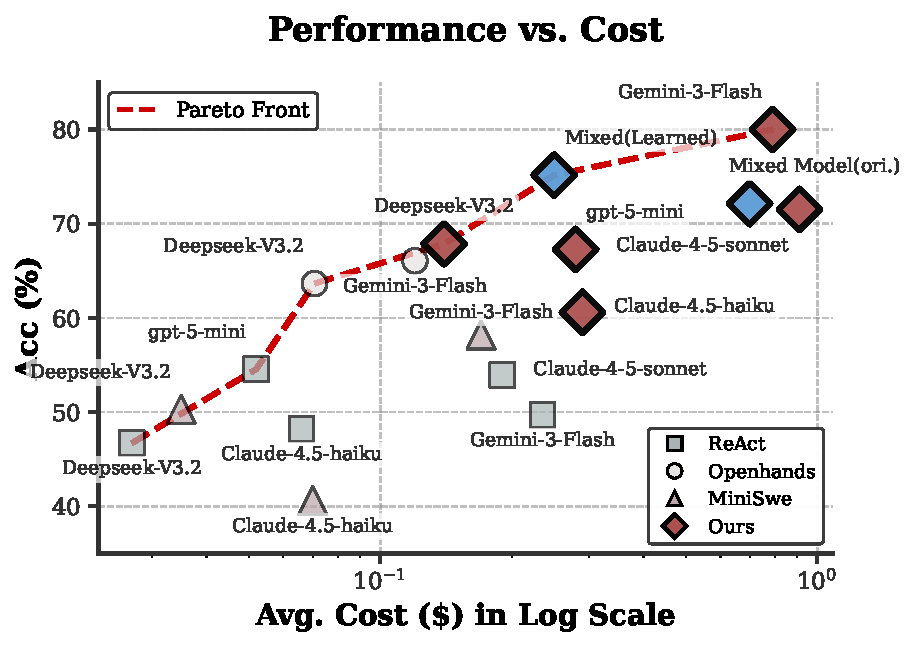
\includegraphics[width=\linewidth]{figures/gaia_cost_performance.pdf}
    \caption{\textbf{GAIA 的帕累托前沿曲线。}图中绘制 GAIA 准确率和每项任务的平均成本（美元，对数刻度）。每个点对应一种配置，虚线表示 \our 在不同模型路由选择下形成的帕累托前沿。}
    \label{fig:cost}
\end{figure}

\paragraph{用于成本感知编排的上下文内学习。}
\our{} 的另一项优势是能够通过逐步模型路由平衡成本与性能。表~\ref{tab:level_main} 表明，使用不同子智能体模型会形成明显不同的准确率与成本曲线，因此编排器必须感知这种权衡。为此，我们采用面向帕累托前沿的上下文学习过程，根据带有性能与货币成本反馈的交互轨迹，迭代优化编排器指令。得到的策略在降低成本的同时改进了 \our：在混合模型设置中，Ours (ICL) 将准确率从 $72.12\%$ 提升至 $75.15\%$，同时把平均成本从 \$0.70 降至 \$0.57（表~\ref{tab:level_main}），说明简单的提示词级学习能够同时提高性能与效率。在系统层面，图~\ref{fig:cost} 进一步表明 \our 可以自然形成帕累托有效的运行点：在不同模型选择下，我们的配置构成帕累托前沿，相比基线系统性地改善了成本与性能的权衡。

\subsubsection{优势三：即插即用的子智能体}
\label{sec:adv3}
本节验证该方法在框架层面的可插拔性。具体而言，我们在 Terminal-Bench 上使用 \texttt{Gemini-3-Flash} 作为编排器，并按照附录~\ref{app:dataset} 的设置，将子智能体的执行后端替换为 ReAct 风格、Mini-SWE 风格等不同智能体框架。

表~\ref{tab:plugin_subagent} 表明，当使用不同的子智能体后端时，\our 仍能保持稳定性能，并持续优于相应基线。该设计使子智能体可以充当即插即用的模块，让系统无需依赖任何特定子智能体实现也能保持稳健。

\begin{table}[]
\centering
\setlength{\tabcolsep}{6pt}
\caption{在固定编排器下评估即插即用的子智能体。我们使用 Gemini-3-Flash 测试不同子智能体实现的稳健性与可复用性。}
\label{tab:plugin_subagent}
\resizebox{\linewidth}{!}{%
\begin{tabular}{l c c c c}
\toprule
\textbf{系统}
& \textbf{简单}
& \textbf{中等}
& \textbf{困难}
& \textbf{准确率} \\
\midrule
\multicolumn{5}{l}{\textbf{独立基线}} \\
\midrule
ReAct                     & 50.00 & 34.09 & 16.67 & 28.57 \\
Mini-SWE-Agent            & 50.00 & 40.91 & 20.83 & 34.29 \\
Claude Code               & 50.00 & 41.86 & 16.67 & 32.86 \\
\midrule
\multicolumn{5}{l}{\textbf{带可插拔子智能体的编排器}} \\
\midrule
ReAct 风格子智能体       & 50.00 & \textbf{63.63} & 20.83 & \textbf{48.57} \\
Mini-SWE 风格子智能体    & \textbf{100.00} & 47.73 & \textbf{33.33} & 44.29 \\
\bottomrule
\end{tabular}
}
\end{table}
